\usepackage[english] {babel}
\usepackage[T1]      {fontenc}

\usepackage{amsmath, amsfonts, graphicx}
\usepackage{bibunits, tikz}
\usetikzlibrary{datavisualization, datavisualization.formats.functions}
\usepackage{pgfplots}
\usetheme{progressbar}

\setbeamersize
  {text margin left=1em, text margin right=1em}

\title
  [Automatic WTB Inspection]
  {Automatic Wind Turbine Blade Inspection}

\author
  [Cesar Gonzalez]
  {Cesar Gonzalez}

\date
  {\today}

\institute
  {}

\begin{document}

\maketitle

\begin{frame}{Overview}

  \tableofcontents

\end{frame}

\section {Motivation}

\subsection{Capacity installed}

  \begin{frame}[fragile] {Wind Energy Capacity installed today} % Using beamer we should specify fragile in order to use datavisualization

%	  \begin{tikzpicture}
%		  \begin{axis}[
%			width = 10cm, height=6cm,
%			grid = major,
%			grid style={dashed, gray!30},
%			axis background/.style={fill=white},
%			ylabel= Gigawatts,
%			xlabel= Year,
%			/pgf/number format/.cd,
%			use comma,
%			1000 sep={},
%		tick align = outside]
%		\addplot table []{data/Capacityinstalled.csv};
%	\end{axis}
%\end{tikzpicture}
\begin{figure}[!h]
\centering

\begin{tikzpicture}[scale=0.9]
	\begin{axis}
		[title=Capacity Installed,
		 xlabel={Year},
		 ylabel={Gigawatts},
		 /pgf/number format/.cd, % To display the years correctly
		 1000 sep={},
		 ybar,
		 bar width=7pt, % Separation between bars
	 ]
	 \addplot[blue!20!black, fill=blue!80!white]  table {data/Capacityinstalled.csv};
	\end{axis}
\end{tikzpicture}

\end{figure}
\end{frame}

\subsection{WTG Blade Faults}

\begin{frame}{Blade Faults and Unavailability}
	\begin{columns}[T]
	\begin{column}{4.5cm}
		Most common faults of blades:	
		\begin{itemize}

			\item Delamination
			\item Fatigue
			\item Lightning damage
			\item Cracks
			\item Lack of glue
			\item Others

		\end{itemize}
	\end{column}
	
	\begin{column}{6cm}
		Unavailability
		\begin{figure}[!h]
			\centering
			\begin{tikzpicture}[scale=0.7]
				\begin{axis}
				[title=Contribution to Unavailability,
		 		ylabel=\%,
		 		/pgf/number format/.cd, % To display the years correctly
		 		1000 sep={},
				xticklabels from table={data/CUnavailability.csv}{System},
				xtick=data,
				ybar,
				x tick label style={rotate=75, anchor=east}
		 		 % Separation between bars
	 			]
				\addplot  [blue!20!black, fill=blue] table[ x expr=\coordindex, y=Contribution] {data/CUnavailability.csv};
				\end{axis}
			\end{tikzpicture}
		\end{figure}
	\end{column}
	\end{columns}
\end{frame}

\subsection{Difficult Maintenance}

\begin{frame}{Maintenance}
	
\end{frame}

\section{The idea}

\begin{frame}{The solution proposed}

\end{frame}
%\begin{frame}
%  {Pictures}
%
%  \begin{figure}[t]
%    \centering
%    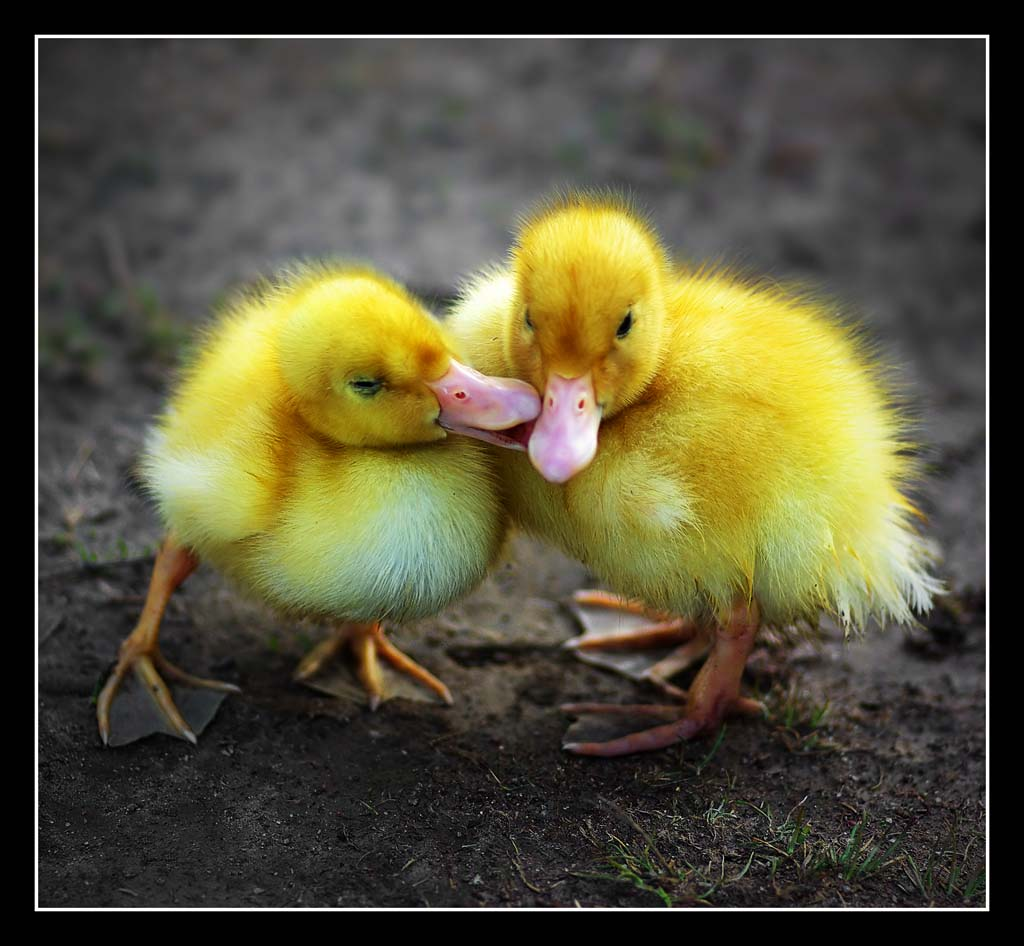
\includegraphics[height=\dimexpr11\textheight/16\relax]{ducks}
%    \caption{Kissing ducks}
%  \end{figure}
%\end{frame}
%
%
%\begin{frame}
%  {A Movie}
%
%  \begin{block}
%    {Some block}
%
%    \begin{itemize}
%    \item Movies only seem to work in Adobe Reader
%    \item Movie file is not embedded, it must be on the computer
%    \end{itemize}
%  \end{block}
%
%  \pause
%  \begin{alertblock}
%    {Some more block}
%
%    Movies only seem to work in Adobe Reader\par
%    Movie file is not embedded, it must be on the computer
%  \end{alertblock}
%  \pause
%
%  \begin{exampleblock}{}
%    Some text in here.
%
%    \begin{itemize}[<+->]
%    \item Movies only seem to work in Adobe Reader
%    \item Movie file is not embedded, it must be on the computer and
%      what happe with a very long item?
%    \end{itemize}
%  \end{exampleblock}
%\end{frame}


\section
  {Questions}

  \begin{frame}{Questions}
	  \centering
	Any questions?
  \end{frame}
%\begin{bibunit}[plain]
%\begin{frame}
%  {Credits}
%
%  \begin{itemize}
%  \item Brought to you by Cédric Mauclair
%  \item Please let me know about improvements!
%  \item Inspiration: \url{http://www.shawnlankton.com}... (in code)
%  \end{itemize}
%
%  \nocite{ipsum}
%  \bibliography{demo}
%
%\end{frame}
%\end{bibunit}
%
%\begin{bibunit}[plain]
%\begin{frame}
%  {Questions}
%
%  \nocite{lorem}
%  \bibliography{demo}
%
%\end{frame}
%\end{bibunit}
%
\end{document}


%%% Local Variables:
%%% mode: latex
%%% TeX-master: "demo-slides.tex"
%%% End:
